\documentclass[11pt, a4paper]{report}
\usepackage[utf8]{inputenc}
\usepackage[T1]{fontenc}
\usepackage{ngerman}
\usepackage[left=2cm,right=2cm,top=2cm,bottom=2cm]{geometry}
\usepackage{charter}
\usepackage{custompkg}
\usepackage{amsmath}
\usepackage{graphicx}

\begin{document}
	\bsremovechaptertitle
	\title{Exponentialfunktionen Übung}
	\author{Ben Siebert \and Tanel Malak \and Julina Elfert \and Moritz Junkermann}
	\date{\today}
	\maketitle
	\tableofcontents
	\chapter{S. 136 Nr. 3}
	\paragraph{Produktregel:}
	$f'(x) = u'(x) \times v(x) + u(x) \times v'(x)$
	
	\section{Teilaufgabe a)}
	$f(x) = x \times e^x$ \\
	$u_1 = x;\  v_1 = e^x \Rightarrow u_1' = 1;\ v_1' = e^x $ \\\\
	$f'(x) = 1 \times e^x + x \times e^x$ \\
	$\Leftrightarrow f'(x) = e^x \times (1 + x)$ \\
	$u_2 = e^x;\ v_2 = 1 + x;\ u_2' = e^x;\ v_2' =  1$ \\\\
	$f''(x) = u_2' \times v_2 + u_2 \times v_2'$ \\
	$\Leftrightarrow f''(x) = e^x \times (1+x) + e^x \times 1$ \\
	$\Leftrightarrow f''(x) = e^x \times (2+x)$ \\

	\paragraph{Extremstellen} \mbox{} \\
	notwendige Bedingung für EST: $f'(x) = 0$ \\
	$f'(x) = 0 \\
	e^x \times (1 + x) = 0\ \Bigl|\div e^x \\
	1 + x = 0\ \Bigl| -1 \\
	x_1 = -1
	$
	\\
	hinreichende Bedingung für EST: $f'(x) = 0\ \land\ f''(x) \ne 0 $
	\\
	$
	f''(-1) = e^{-1} \times (2 - 1) \\
	f''(-1) = e^{-1} \times 1 \\
	f''(-1) = e^{-1}
	$
	\\
	Y-Koordinate: $f(-1) = -1e^{-1}$
	\\
	Tiefpunkt bei P(-1|$-e^{-1} $)
	
	\section{Teilaufgabe c)}
	$
	f(x) = (4x - 1) \times e^x \\
	u_1 = 4x - 1;\ v_1 = e^x;\ u_1' = 4;\ v_1' = e^x \\\\
	f'(x) = 4 \times e^x + (4x - 1) \times e^x \\
	\Leftrightarrow f'(x) = e^x \times (4x + 3) \\
	u_2 = e^x;\ v_2 = 4x + 3;\ u_2' = e^x;\ v_2' = 4 \\\\
	f''(x) = e^x \times (4x + 3) + e^x \times 4 \\
	\Leftrightarrow f''(x) = e^x \times (4x + 7)
	$
	\\
	\paragraph{Extremstellen} \mbox{} \\
	notwendige Bedingung für EST: $f'(x) = 0$ \\
	$
	f'(x) = 0 \\
	e^x \times (4x + 7) = 0\ \Bigl|\div e^x\\
	4x+7= 0\ \Bigl|-7 \\
	4x = -7\ \Bigl|\div 4 \\
	x = -\frac{7}{4}
	$
	\\
	hinreichende Bedingung für EST: $f'(x) = 0\ \land\ f''(x) \ne 0$ \\
	$
	f''(-\frac{7}{4}) = e^{-\frac{7}{4}} \times (4 \times -\frac{7}{4} + 7) \\
	f''(-\frac{7}{4}) = 0
	$
	\\
	Vorzeichenwechselkriterium (VZW): \\
	$
	f'(-2) = -5e^{-2} \Rightarrow negativ \\
	f'(2) = 11e^2 \Rightarrow positiv \\
	$
	\\
	Y-Koordinate: $f(-\frac{7}{4}) = -8 \times e^{-\frac{7}{4}}$ \\
	Tiefpunkt bei T($-\frac{7}{4}$|$-8 \times e^{-\frac{7}{4}}$)
	\section{Teilaufgabe f)}
	$
	f(x) = x^2 \times e^x \\
	u_1 = x^2;\ v_1 = e^x;\ u_1' = 2x;\ v_1' = e^x \\\\
	f'(x) = 2x \times e^x + x^2 \times e^x \\
	\Leftrightarrow e^x \times (2x + x^2) \\
	u_2 = e^x;\ v_2 = 2x + x^2;\ u_2' = e^x;\ v_2' = 2 + 2x \\\\
	f''(x) = e^x \times (2x + x^2) + e^x \times (2 + 2x) \\
	\Leftrightarrow f''(x) = e^x \times (x^2 + 2 + 4x)
	$
	\\
	\chapter{S. 137 Nr. 5}
	\section{Teilaufgabe a)}
	$f(x) = (3 - x) \times e^{-x}$ \\
	Nullstellen: \\
	$
	f(x) = 0 \\
	(3 - x) \times e^{-x} = 0
	$\\
	Satz vom Nullprodukt: $x_1 = 3$ \\\\
	$
	u_1 = 3 - x;\ v_1 = e^{-x};\ u_1' = -1;\ v_1' = -e^{-x}\\\\
	f'(x) = -1 \times e^{-x} + (3 - x) \times (-e^{-x}) \\
	\Leftrightarrow f'(x) = e^{-x} \times (x - 4) \\
	u_2 = e^{-x};\ v_2 = x - 4;\ u_2' = -e^{-x};\ v_2' = 1 \\\\
	f''(x) = -e^{-x} \times (x - 4) + e^{-x} \times 1 \\
	\Leftrightarrow f''(x) = e^{-x} \times (5 - x) \\
	$
	\section{Teilaufgabe b)}
	notwendige Bedingung für EST: $f'(x) = 0$ \\
	$
	f'(x) = 0 \\
	e^{-x} \times (x - 4) = 0
	$ \\
	Satz des Nullprodukts: $x_1 = 4$ \\
	hinreichende Bedingung für EST: $f'(x) = 0\ \land\ f''(x) \ne 0$\\
	$
	f''(4) = e^{-4} \Rightarrow positiv \to TP\\
	$
	Y-Wert: $f(4) = -e^{-4}$
	\\
	Der Graph der Funktion $f$ hat einen Tiefpunkt $T(4\Bigl|-e^{-4})$ \\
	\section{Teilaufgabe c)}
	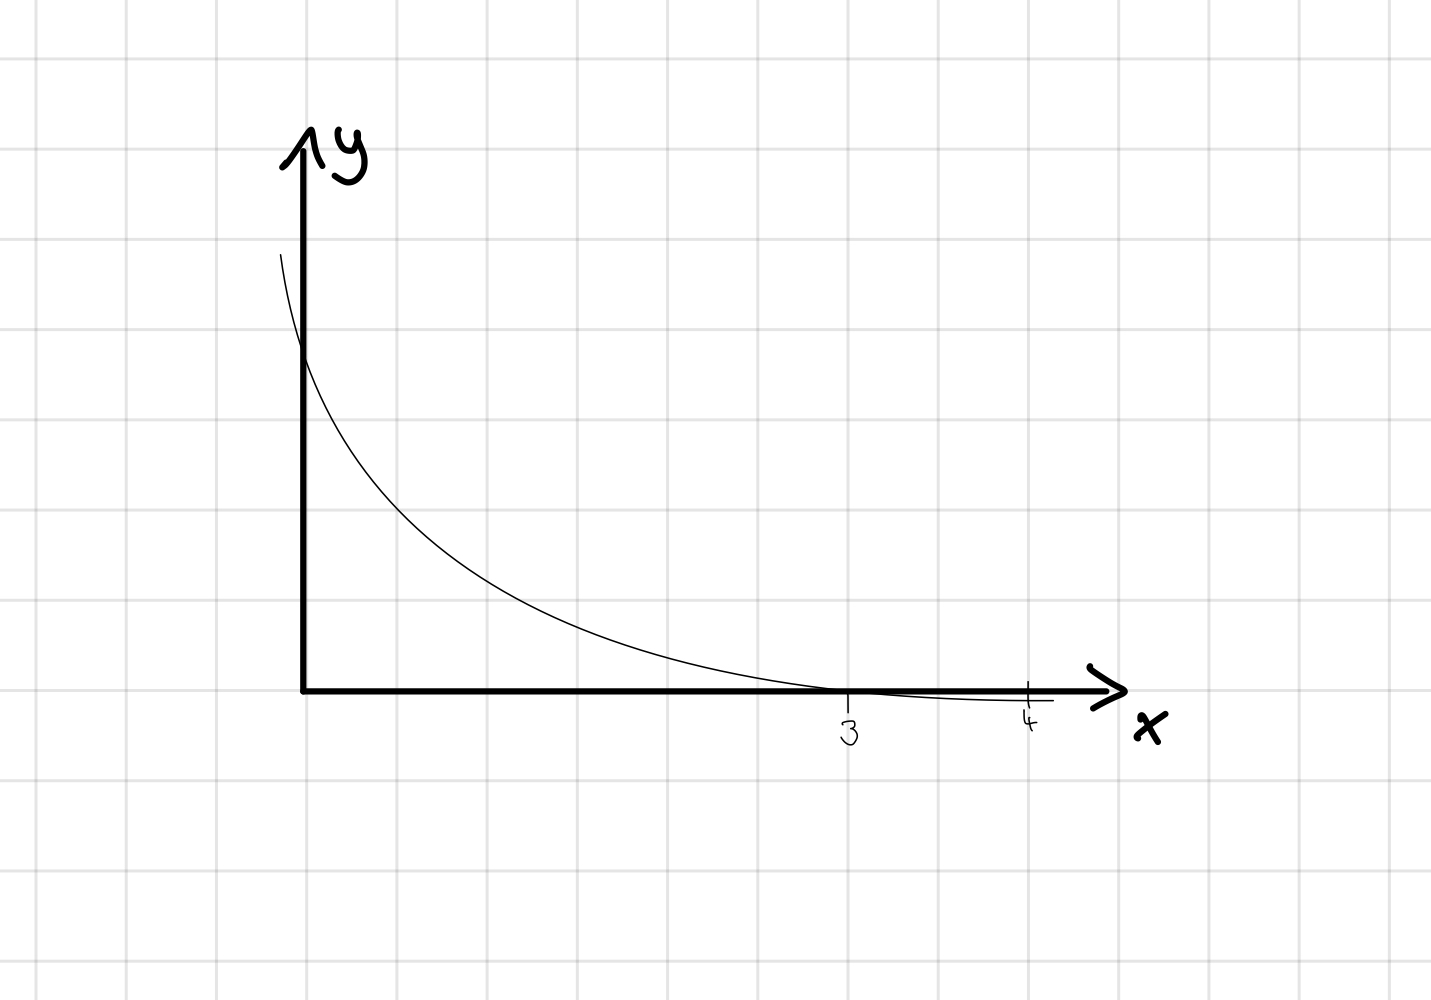
\includegraphics[width=10cm]{SKIZZE.JPEG}
	\section{Teilaufgabe d)}
	$
	t(x) = mx + b \\
	m = f'(0) = -4 \\
	t(0) = -4 \times 0 + b = 3 \\
	\Leftrightarrow b = 3 \\
	t(x) = -4x + 3
	$
	\chapter{S. 139 Nr. 1}
	\section{Teilaufgabe a)}
	$
	f(x) = (x + 2)^4\\
	u^\circ v\\
	u=x^4;\ v=x + 2;\ u' = 4x^3;\ v' = 1 \\
	f'(x) = u'(v(x)) \times v'(x) \\
	\Leftrightarrow f'(x) = 4 \times (x + 2)^3 \times 1 \\
	\Leftrightarrow f'(x) = 4 \times (x + 2)^3 \\
	$
	\section{Teilaufgabe e)}
	$
	f(x) = e^{2x} \\
	u^\circ v \\
	u = e^x;\ v= 2x;\ u' = e^x;\ v' = 2 \\
	f'(x) = u'(v(x)) \times v'(x) \\
	\Leftrightarrow f'(x) = e^{2x} \times 2 \\
	\Leftrightarrow f'(x) = 2e^{2x}
	$
	\chapter{S. 139 Nr. 2}
	\section{Teilaufgabe a)}
	$
	f(x) = 2e^{x^3-x^2}\\
	u^\circ v\\
	u = 2e^x;\ v= x^3-x^2;\ u' = 2e^x;\ v' = 3x^2-2x \\
	f'(x) = 2e^{x^3-x^2} \times (3x^2-2x)\\
	f'(x) = (6x^2 - 4x) \times e^{x^3 - x^2}
	$
	\section{Teilaufgabe b)}
	$
	f(x) = e^{\sqrt{x}} \\
	u = e^x;\ v = \sqrt{x};\ u' = e^x;\ v' = \frac{1}{2 \times \sqrt{x}} \\
	f'(x) = e^{\sqrt{x}} \times \frac{1}{2 \times \sqrt{x}} \\
	\Leftrightarrow f'(x) = \frac{e^{\sqrt{x}}}{2\times \sqrt{x}}
	$
	
	\section{Teilaufgabe g)}
	$
	f(x) = 3x \times ln(2x) \\
	u = 3x;\ v = ln(2x) = ln(2) + ln(x);\ u' = 3;\ v' = \frac{1}{x} \\
	f'(x) = 3 \times ln(2x) + 3x \times \frac{1}{x} \\
	f'(x) = 3 \times (ln(2x) + 1)
	$
	
	\section{Teilaufgabe h)}
	$
	f(x) = ln(\sqrt{x}) \\
	u^\circ v\\
	u = ln(x);\ u' = \frac{1}{x};\ v = \sqrt{x};\ v' = \frac{1}{2 \times \sqrt{x}} \\
	f'(x) = \frac{1}{\sqrt{x}} \times \frac{1}{2 \times \sqrt{x}} \\
	\Leftrightarrow f'(x) = \frac{1}{2x}
	$
	
	\chapter{S. 139 Nr. 5}
	$
	f(x) = (2x - 1)^2 \times e^x
	$
	\section{Teilaufgabe a)}
	$
	u = e^x;\ u' = e^x;\ v = (2x - 1)^2 = 4x^2 - 4x + 1;\ v' = 8x - 4 \\
	f'(x) = e^x \times (8x - 4) + e^x \times (4x^2 - 4x + 1) \\
	f'(x) = e^x \times (8x - 4 + 4x^2 - 4x + 1) \\
	f'(x) = e^x \times (4x - 3 + 4x^2) \\
	$
	\\
	Steigung im Punkt $P\Bigl(2\Bigl|f(2)\Bigl)$ \\
	$
	f'(2) = e^2 \times (4 \times 2  - 3 + 4\times 2^2) \\
	\Leftrightarrow e^2 \times 21 \\
	$ \\
	Die Steigung im Punkt $P\Bigl(2\Bigl|f(2)\Bigl)$ liegt bei $21 \times e^2$
	\\
	\section{Teilaufgabe b)}
	$
	t(x) = mx + b\ \Bigl|\ m = 0 \to waagerecht \\
	\Rightarrow t(x) = b \\
	$
	notwendige Bedingung für EST: $f'(x) = 0$ \\
	$
	f'(x) = 0 \\
	\Leftrightarrow e^x \times (4x - 3 + 4x^2) = 0 \\
	\Rightarrow 4x - 3 + 4x^2 = 0\ \Bigl|\div 4 \\
	\Rightarrow x - \frac{3}{4} + x^2 = 0 \\
	p.q.\Rightarrow x_1,x_2 =  -\frac{p}{2} \pm \sqrt{(\frac{p}{2})^2 - q} \\
	\Leftrightarrow x_1,x_2 = -\frac{1}{2} \pm \sqrt{(\frac{1}{2})^2 + \frac{3}{4}} \\
	\Leftrightarrow -\frac{1}{2} \pm \sqrt{\frac{1}{4} + \frac{3}{4}} \\
	\Leftrightarrow -\frac{1}{2} \pm \sqrt{\frac{4}{4}} \\
	\Leftrightarrow -\frac{1}{2} \pm \sqrt{1} \\\\
	\Leftrightarrow -\frac{1}{2} \pm 1 \\
	\Rightarrow x_1 = \frac{1}{2};\ x_2 = -\frac{3}{2}
	\\
	$\\
	hinreichende Bedingung für EST: $f'(x) = 0 \land VZW$ \\
	\begin{align}
		\left.x_1:
		\begin{array}{ll}
			f'(\frac{1}{4}) = e^{\frac{1}{4}} \times (4\times \frac{1}{4} - 3 + 4\times \frac{1}{4}^2)\\
			 = e^{\frac{1}{4}} \times (1 - 3 + \frac{1}{4}) \\
			 = e^{\frac{1}{4}} \times (-\frac{7}{4}) \\
			 \\
			 f'(\frac{3}{4}) = e^{\frac{3}{4}} \times (4\times \frac{3}{4} - 3 + 4\times \frac{3}{4}^2)\\
			 = e^{\frac{3}{4}} \times (3 - 3 + 4 \times \frac{9}{16}) \\
			 = e^{\frac{3}{4}} \times (\frac{9}{4}) \\
		\end{array}
		\right\} negativ/positiv\ VZW\ \to TP
	\end{align}
	\begin{align}
		\left.x_2:
		\begin{array}{ll}
			f'(-2) = e^{-2} \times (4\times (-2) - 3 + 4\times (-2)^2)\\
			 = e^{-2} \times (-8 - 3 + 16)\\
			 = e^{-2} \times 5\\
			 \\
			 f'(0) = e^{0} \times (4\times 0 - 3 + 4\times 0^2)\\
			 = - 3
		\end{array}
		\right\} positiv/negativ\ VZW\ \to HP
	\end{align}
	\\
	Y-Koordinaten bestimmen: \\\\
	$
	x_1: f(x_1) = f(0.5) = (2 \times 0.5 - 1)^2 \times e^{0.5} = 0 \\
	x_2: f(x_1) = f(-1.5) = (2 \times (-1.5) - 1)^2 \times e^{-1.5} = (-4)^2 \times e^{-1.5} = 16 \times e^{-1.5}
	$
	\\\\
	Die Funktion $f(x)$ hat einen Tiefpunkt $TP\Bigl(0.5\Bigl|0\Bigl)$ und eine Hochpunkt $HP\Bigl(-1.5\Bigl|16 \times e^{-1.5}\Bigl)$ \\
	Die Tangenten der Extremstellen verlaufen waagerecht, also parallel zur X-Achse: \\
	$
	t_1(x) = 0 \\
	t_2(x) = 16 \times e^{-1.5}
	$
	
	\chapter{S. 140 Nr. 9}
	$
	f(x) = \frac{2}{(1+2x)^2} \\
	f'(x) = \frac{-8}{(2x+1)^3}
	$
	\section{Teilaufgabe a)}
	$
	(1 + 2x)^2 = 0 \\
	(1 + 2x) \times (1 + 2x) = 0 \\
	1 + 2x = 0 \\
	2x = -1 \\
	x = -0.5 \\
	$
	Die Funktion ist für $x = -0.5$ nicht definiert. \\
	$
	x \in \rm I\!R\ \backslash\ \{-0.5\}
	$
	\section{Teilaufgabe b)}
	streng monoton abnehmend: $f'(x) < 0$: \\
	$f'(x)$ ist kleiner als null, solange $2x +1$ positiv ist. \\
	$2x + 1$ ist positiv, wenn $x > -0.5$ \\\\
	$
	x \in \rm I\!R\ > -0.5
	$
	\section{Teilaufgabe c)}
	$f(x)$ kann keine Extremstellen haben, da die Ableitung $f'(x)$ niemals gleich null ist.
	Da es ein Bruch ist, ist die Stelle, bei der der Nenner gleich null ist, nicht definiert.
	
	\section{Teilaufgabe d)}
	$
	t(x) = mx + b \\
	f(0) = \frac{2}{(1+2 \times 0)^2} = \frac{2}{1} = 2 \\
	\Rightarrow P(0|2) \\
	f'(0) = -8 \\
	t(x) = -8x + 2
	$
	

	
\end{document}